\documentclass[12pt]{article}

\usepackage{sbc-template}
\usepackage[brazil,american]{babel}
\usepackage[utf8]{inputenc}

\usepackage{graphicx}
\usepackage{url}
\usepackage{float}
\usepackage{listings}
\usepackage{color}
\usepackage{todonotes}
\usepackage{algorithmic}
\usepackage{algorithm}
\usepackage{hyperref}
\usepackage{indentfirst}
\usepackage[inline]{enumitem}

\graphicspath{{./images/}}

\sloppy

\title{Laboratório 2\\- ULA e FPULA –}

\author{GRUPO 6\\
	Dayanne Fernandes da Cunha, 13/0107191\\
	Lucas Mafra Chagas, 12/0126443\\
	Marcelo Giordano Martins Costa de Oliveira, 12/0037301\\
	Lucas Junior Ribas, 16/0052289\\
	Caio Nunes de Alencar Osório, 16/0115132\\
	Diego Vaz Fernandes, 16/0117925}

\address{Dep. Ciência da Computação -- Universidade de Brasília (UnB)\\
  CiC 116394 - OAC - Turma A
  \email{}
}

\begin{document}
\maketitle

\section{Objetivos}
\label{sec:Objetivos}

\begin{itemize}
\item Introduzir ao aluno a Linguagem de Descrição de \textit{Hardware Verilog};
\item Familiarizar o aluno com a plataforma de desenvolvimento \textit{FPGA DE2} da \textit{Altera} e o \textit{software QUARTUS-II};
\item Desenvolver a capacidade de análise e síntese de sistemas digitais usando \textit{HDL}.
\end{itemize}

\section{Ferramentas}
\label{sec:Materiais}

\begin{itemize}
\item FPGA DE2 da Altera 
\item QUARTUS-II
\item Verilog
\item HDL
\end{itemize}

\section{Exercícios}
\label{sec:exercicios}

Todos os códigos escritos neste laboratório podem ser encontrados no repositório \url{https://github.com/Dayof/OAC172} do \textit{GitHub}.

\subsection{Exercício 1. Implementação de um \textit{driver} para \textit{display} de 7 segmentos}
\label{subsec:1driver}

Conforme descrito no arquivo \textit{QuartusIIv3.txt} e \textit{Set.txt}, um novo projeto foi criado no diretório \textit{Display}.

%\begin{figure}[H]
%	\centering
%	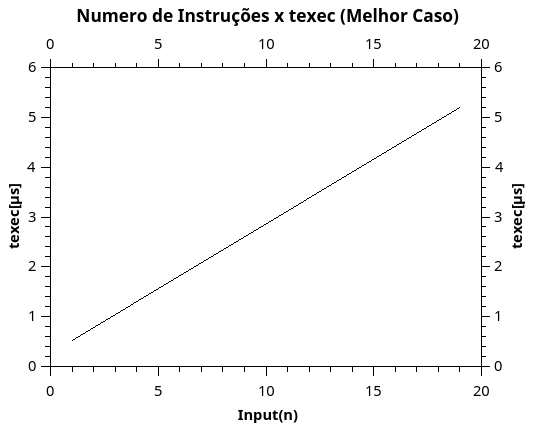
\includegraphics[width=.8\textwidth]{txnMC.png}
%	\caption{n x texec(Melhor Caso)}
%	\label{fig:txnMC}
%\end{figure}

\subsection{Exercício 2. Unidade Lógica Aritmética de Inteiros}
\label{subsec:ulaint}

\subsection{Exercício 3. Unidade Aritmética de Ponto Flutuante }
\label{subsec:ulafloat}

\bibliographystyle{sbc}
\bibliography{relatorio}

\end{document}
